% !TeX program = xelatex
% !TeX encoding = UTF-8
\documentclass{MathModeling}
\usepackage{mwe,color,float}
\usepackage[linesnumbered,ruled]{algorithm2e}
\usepackage{setspace}
\usepackage{colortbl}
\usepackage{tablefootnote}
\usepackage{hyperref}
\everymath{\displaystyle}

\begin{document}
\setcounter{page}{1}
\pagestyle{fancy}

	\section{问题的提出组内赛期分工——建模手、编程手、论文手}
	建模手:数据预处理$+$数据重组$+$问题一的求解

	编程手:数据预处理$+$问题二的求解$+$模型查找

	论文手:论文撰写$+$模型原理查找$+$论文整合
	
	\section{完成任务质量——论文书写排版、python代码、LaTeX代码}
	此次比赛中,我们小组暴露出了很多问题,如论文书写排版、python代码、Latex代码方面上,以下为部分问题及其改正方式。

	\subsection{论文书写排版:}
	1.背景欠缺,使用的方法未具体

	\textbf{\textcolor{red}{例:}}为了预测未来用户的使用软件概率及使用软件频率, 现就部分用户的已知数据进行,通过聚类,分类,回归,预测等方法,对其进行分析。

	\textbf{\textcolor{red}{改:}}为预测未来用户的使用软件概率及使用软件频率,现就部分用户的已知数据进行K-means聚类、随机森林分类、决策树预测,并对结果进行分析。
	
	2.关键词拟定欠佳

	\textbf{\textcolor{red}{例:}}关键词:数据重组;K-means;随机森林;决策树
	关键词在论文中起点睛作用,应该慎重选择,且贴合文章的内容。

	\textbf{\textcolor{red}{改:}}关键词:数据重组、K-means用户聚类、模型比较、随机森林、决策树
	
	3.摘要中只需要结果,并不需要“具体的分析见下文”,如确实需要需做交叉应用

	\textbf{\textcolor{red}{例:}}利用肘部法则并将其可视化,我们确定了K-means聚类的 $k$值为5;最后我们绘制了聚类散点图,并对其分析,具体分析见下文。

	\textbf{\textcolor{red}{改:}}我们通过肘部法则可视化确定了k值为5:并绘制了聚类散点图展开相应的分析(具体结果见于……做交叉引用)
	
	4.题目、摘要、关键词为摘要专用页,仅能一页。
	
	5.摘要结构不清晰,较为繁琐 
	
	\textbf{\textcolor{red}{例:}}
	针对问题一(一)……,

	针对问题一(二)……,

	针对问题一(二)……,

	针对问题一(二)……,
	
	\textbf{\textcolor{red}{改:}}
	针对问题一……,

	针对问题二……,
	
	6.PDF第一页设定初始页码存在问题,原因在于摘要并未集中在一页上。

	7.图形缩放比例不佳,在比较两个图的时候我们应该将图片排成一排,如
	\begin{figure}[H]
		\centerline{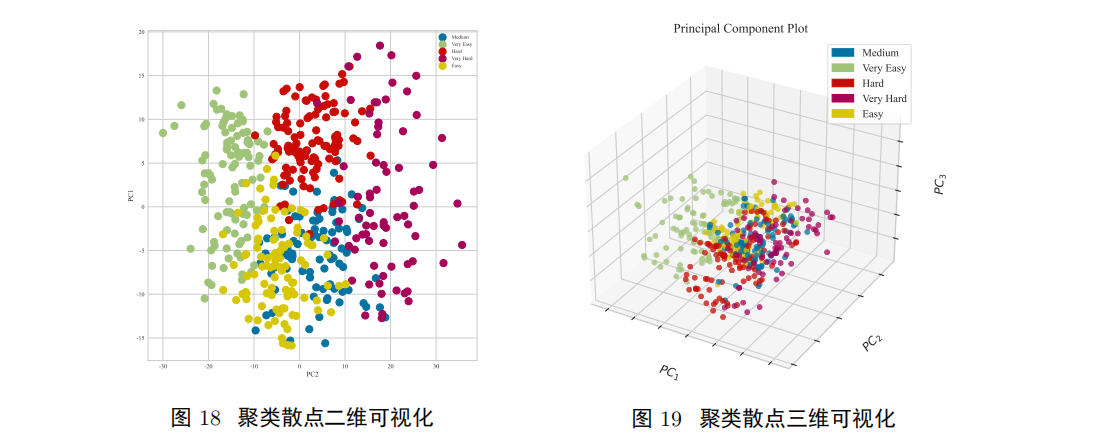
\includegraphics[scale=0.8]{图片1.png}}
	\end{figure}

	8.我们的论文中出现表格过多,应统一为一种表格,如三线表,且表格的样式可以根据实际情况改变。

	9.文章层次不清晰,可能的原因在于全文大多为宋体,如标题一类的需黑体加粗,这次因时间缘故并未做好。

	\subsection{python代码:}
	1.部分语句未遵循PEP8规范。

	导入模块应该放在文件顶部,按字母顺序导入。

	运算符两侧各保留一个空格,逗号后面保留一个空格。

	函数和类定义之间空两行,方法定义之间空一行。

	每个语句块后面要加空行。
	
	2.注释应该完整的阐述代码的功能和意图。
	$$
	{df_1}=df.drop\left(\left['start\_day', 'end\_day', 'Unnamed:0','uid', 'start\_time', 'end\_time', 'app\_type'\right],axis=1\right)
	$$
	$df_1$应该加上注释\#去掉()列
	
	3.输出的pdf图片部分西文字体未修改
	
	安装或引用wand库,wand库会自动检测图片中的文字框,通过text\_boxes属性可以获取到文字框列表,然后设置每个文字框的font属性为Times New Roman,这样就可以批量将中西文字体改为Times New Roman。
	
	4.没有提前考虑数据的合理性,对于数据出现的召回率较低,正类预测效果较差的问题没有解决。
	
	5.重复任务复制粘贴耗时过长,应利用好def进行封装,提高效率。

	如果需要打印的字符串很多,就可以利用def封装成函数,这样以后每次需要,就可以直接调用函数,而不用重复编写代码,提高了代码的复用性和编程效率。
	
	\subsection{LaTeX代码:}
	1.公式的正体斜体区分不标准,内容较多,故附网址:\href{https://blog.csdn.net/wanjiac/article/details/106085105}{https://blog.csdn.net/wanjiac/article/details/106085105}

	2.文中未使用过{\heiti 黑体加粗},而全部为\textbf{宋体}加粗。

	3.三线表有一部分文字不能做到居中对齐。三线表尺寸比例不合理,过长或者过短。

	4.图片比例不合理。一些同类型的图片可以两张并列放置。

	5.附录的python代码需要做好标注。

	6.公式内波浪号:$\sim$,正文内波浪号: \textasciitilde,论文内未正确使用。
	\section{组会纪要}
	1.为了保证论文完整度,需要三个人全程参与,且完成后要有人负责检查。

	2.三个人的进度应保持一致,此次比赛中,我们没有做到这一点。

	3.论文切忌假大空,套用模型时需要有自己的理解,并不能把原理直接往上面抄写,需要有自己的内容分析。

	4.要学会熟练使用文献检索,不单单是知网,有的时候数学建模比赛的题目来源于他人的优秀论文,可以通过文件检索、百度学术、谷歌等查询,查询源文件可以将其转换为英文查询。

	5.对于模型的比较我们可以做一个表格集中体现,方便评委阅读,也显得比较整洁。

	6.题目的拟定很重要,要与论文内容息息相关,能明确地凸显出主题。比赛中最重要的就是论文,故完成初稿后,需要检查、排版、色彩搭配、标点符号等方面的问题。

	7.绘制图像表格时需要给图表命名一个标题,注意标题的位置为表上图下,图表中还要包括对$x$,$y$轴的定义等内容。

	8.最后有时间的话需要对论文进行降重处理,如将一些内容绘制成流程图,这也会是加分点。

	9.引用文献时需注意规范,对引用文献的地方做好标注和交叉引用,需学会网页的引用,并做成超链接。

	\section{体会}
	\textbf{张:}

	怎么说呢,这次比赛完成的过于仓促,我感觉并没有发挥出我们的真实水平,主要原因在于我没有合理的安排好时间,造成了前松后紧的情况,前面三天我们其实已经初步建立了大概思路,但因数据体量较大,后续建模无法进行,在第四天的时候我们决定重新开始,并且比赛期间三个人并没有进行密切的交流,导致三人进度不一样。我也没有给论文手布置好相应任务,导致最后论文结束的过于仓促,且存在很多排版问题,没有时间进行优化。结果就是不仅觉得很累,而且结果也不理想,只能说我要学的东西还很多,接下来一个月我需要用于转专业复习,我大概会在转专业考试后继续对数学建模的学习。

	\textbf{陈:}
	
	时间有点紧张,完事儿感觉后面做的有点混乱了。完成论文的时候就是想到什么做什么,没有什么条理性了,匆忙到交论文前两分钟我还在删半角符号……然后这次前期的讨论啥的也没怎么参与,我全程就是很懵,焦虑但帮不上忙TAT。然后这次也是拼凑的论文,割裂感也好强

	\textbf{许:}
	
	这次比赛感觉使不上力气,数据预处理难度较大,我只是通过张队处理好的数据进行解决问题,但是整理出的数据效果并不好,时间紧张、程序运行复杂的情况下,只在运行效果较差的思路进行分析,没有找到能够优化数据的方法。
\end{document}